\section{Molekulardynamik}

Molekulardynamik (MD) ist im Gegensatz zu quantenmechanischen Methoden eine klassische atomistische Methode, die zwar ungenauere Ergebnisse liefert, jedoch größere Systeme von bis zu einer Million Atome in akzeptabler Zeit rechnen kann.
Damit wird sie seit vielen Jahren erfolgreich in Physik, Chemie sowie in Materialwissenschaften genutzt, um System-, Molekül- und Materialeigenschaften zu bestimmen und Rückschlüsse auf reale Prozesse zu führen.
Somit existiert es eine Vielzahl gut erforschter Systeme, auf die im Rahmen dieser Arbeit aufgebaut wird.

\subsection{Formulierung}

\subsubsection{Allgemeines}

Als klassische Methode arbeitet Molekulardynamik mit Kraftfeldern, Massen.
So besteht ein System aus einer Vielzahl an Teilchen, die als Punktmasse angenähert werden, sowie einer universellen Zeit $t$.
Jedes Teilchen vereint also die Eigenschaften seiner Masse $m$, seines Impulses $\vec p$ und seiner Position $\vec r$.
Zusätzlich wirkt auf jedes Teilchen ein Kraftfeld $F(R)$ mit $R$ als aktuellem Systemzustand.

\subsubsection{Mikrokanonisches Ensemble (NVE)}

Es gilt für jedes Teilchen:

\begin{equation}
  \dot{\vec r} = {\vec p \over m}
\end{equation}

\begin{equation}
  \dot{\vec p} = m \vec a = F(R)
\end{equation}

\todo{Globale Formulierung!}

Zentral ist also das Kraftfeld $F(R)$, welches auf unterschiedliche Arten

\subsubsection{Kanonisches Ensemble (NVT)}

Gegenüber dem mikrokanonischen Ensemble kommt im Kanonischen Ensemble noch ein Thermostat hinzu.
Dieses gleicht die mittlere Temperatur des Systemes an einen vorgegebenen Wert an.
Dies kann über harte Reskalierung der Partikelgeschwindigkeiten (Berendsen-Thermostat), durch zufällige Stöße mit virtuellen Teilchen (Anderson-Thermostat) geschehen, oder durch einen zusätzlichen Reibungsterm, der auch negative Reibungskoeffizienten zulässt (Nosé-\-Hoover-\-Thermostat).

Unter Benutzung des \textbf{Berendsen-Thermostates} werden jeden Zeitschritt die Geschwindigkeiten aller Teilchen so skaliert, dass die Temperatur, die sich aus der kinetischen Energie über die Maxwell-Boltzmann-Verteilung für Gase ergibt, auf dem Zielwert gehalten wird:

\begin{equation}
  \overline{E_{kin}} = {1\over2} m\overline{v^2} = {d\over2}k_BT
\end{equation}

%% \begin{equation}
%% T = {m \overline{v^2} \over k_B d}
%% \end{equation}

Da dabei eine feste Temperatur erzwungen wird, ergibt dieses Thermostat kein kanonisches Ensemble, ist jedoch für große Systeme eine gute Näherung, die effizient berechnet werden kann.

Das \textbf{Anderson-Thermostat} hingegen arbeitet näher an der Idee des kanonischen Ensembles, über die Systemgrenzen hinweg Energie und somit Temperatur durch Teilchenstöße auszutauschen.
Dabei wird für die Zahl der Stöße pro Zeitschritt eine Poissonverteilung angenommen, Masse und Geschwindigkeiten der virtuellen Atome entsprechen der Zieltemperatur.
Zwar hat diese Vorgehensweise den Vorteil, mit einer geringen Anzahl an äußeren Einflüssen die Temperatur konstant zu halten, jedoch eignet es sich nur für die Betrachtung zeitgemittelter Größen.
Durch die Manipulation einzelner, zufälliger Atome können Trajektorien, insbesondere Abscheidungsorte und -konfigurationen stark beeinflusst werden.

Als Alternative eignet sich das \textbf{Nosé-Hoover-Thermostat}.
Dieses fügt dem Gesamtsystem einen zusätzlichen Freiheitsgrad $s$ hinzu, der die Temperatur beeinflusst.
Auf jedes Atom $i$ wirkt somit eine zusätzliche Reibungskraft entlang des Impulses:

\begin{equation}
  \dot{\vec p_i} = \vec{F_i} - s \vec{p_i}
\end{equation}

Der Reibungskoeffizient $s$ ändert sich dabei in Abhängigkeit vom System und kann dabei auch negative Werte annehmen:

\begin{equation}
  \dot s = {\tau \over M} \sum_i{{p_i^2 \over 2m_i} - {Nd \over k_BT}}
\end{equation}

\todo{tau hin oder weg?}

Damit fluktuiert die Temperatur um den Zielwert, wird also nicht fest erzwungen und folgt somit dem kanonischen Ensemble, wobei $\tau$ die Zeitskala angibt, auf der das System ins thermische Gleichgewicht übergeht.
In vielen Softwarepaketen für Molekulardynamiksimulationen dient das Nosé-Hoover-Thermostat als Standardthermostat.

\subsubsection{Großkanonisches Ensemble (NPT)}

Zusätzlich zu einem Thermostat kommt im großkanonischen Ensemble ein Barostat zum Einsatz.
Dieses reguliert über Reskalierung des Simulationsraumes unter periodischen Randbedingungen den mittleren Druck des Systemes.
Dadurch lassen sich periodische Strukturen wie Kristalle frei relaxieren, ohne ihnen eine feste Dichte aufzuzwingen.
Andererseits lassen sich auch Systeme unter großen Drücken untersuchen.

Die Methoden des Barostats gleichen dem des Thermostats, wobei hier nicht die einzelnen Atome, sondern deren relativer Abstand zu einander durch Skalierung der Hauptachsen manipuliert wird.
Als Voreinstellung kommt üblicherweise wieder ein Nosé-Hoover-Barostat zum Einsatz, wobei aufgrund seiner Einfachheit auch Berendsen-Barostate genutzt werden.
Der Druck wird dabei über die Virialgleichung \todo{für ideale Gase?} ermittelt:

\begin{equation}
  PV = Nk_BT + \frac{1}{d} \sum_{i=1}^N{\vec{r}_i \cdot \vec{F}_i}
\end{equation}

\subsubsection{Minimierung durch Konjugierte Gradienten (CG-Minimierung)}

\begin{figure}
  \centering
  \def\svgwidth{0.5\textwidth}
  \input{img/cg-gradient.pdf_tex}
  \caption[CG-Methode]{Klassische Minimierung durch konjugierte Gradienten:\\
    a) Optimale Schrittlänge\\
    b) Kleine Schrittlänge $\Rightarrow$ viele unnötige Schritte\\
    c) Große Schrittlänge $\Rightarrow$ langsames Konvergenzverhalten
  }
  \label{fig:cg-gradient}
\end{figure}

Zur Energieminimierung, welche der Strukturoptimierung dient, wird häufig die \textbf{Methode der konjugierten Gradienten} angewandt.
Man sucht dabei in der grundlegenden Variante ausgehend von einem beliebigen Startpunkt $\vec x_0$ das Minimum der im Suchbereich stetigen Funktion $f(\vec x)$ durch schrittweise Annäherung entlang des Gradienten:

\begin{gather}
  \vec s_i = \Delta\vec x_i = \nabla f(\vec x_{i-1})\\
  \vec x_i = \vec x_{i-1} - \alpha \vec s_i
\end{gather}

Der zusätzliche Parameter $\alpha$ legt dabei die Schrittweite fest.
Mögliche Abbruchkriterien können dabei die Differenz zwischen zwei Schritten ($\left|\vec x_i - \vec x_{i-1}\right| < x_\text{tol}$), die maximale Änderung eines Vektorelementes ($\max_k{\left|x_{i,k} - x_{i-1,k}\right|} < x_\text{tol}$), die Stärke des Gradienten ($\left|\nabla f(\vec x_{i-1})\right| < x_\text{tol}$), eine Anzahl an Zeitschritten ($i > i_\text{tol}$) oder eine Kombination daraus sein.

Dieser grundlegende Algorithmus stößt schnell an seine Grenzen, wenn man allgemeine, nichtlineare Funktionen minimieren möchte.
Dafür führt man mehrere Änderungen ein:
Einerseits ersetzt man den Sprung durch eine Minimierung entlang der Schrittrichtung (Gleichungen \ref{eq:cg-linesearch1} und \ref{eq:cg-linesearch2}).
Andererseits ändert man die Schrittrichtung in Abhängigkeit vorheriger Schritte leicht ab (Gleichungen \ref{eq:pr1} und \ref{eq:pr2}).
Hier wird die Polak-Ribière-Variante vorgestellt1, die standardmäßig in LAMMPS zum Einsatz kommt, jedoch existieren weitere gleichwertige Methoden.

\begin{gather}
  \label{eq:cg-linesearch1}
  \min_\alpha f(x_i+\alpha \vec s_i) \rightarrow \alpha_i \\
  \label{eq:cg-linesearch2}
  \vec x_i = \vec x_{i-1} - \alpha_i \vec s_i\\
  \label{eq:pr1}
  \vec s_i = \Delta \vec x_i + \beta_i \vec s_{i-1}\\
\end{gather}
\begin{equation}
  \label{eq:pr2}
  \beta_i = \max \left(0, \frac{\Delta \vec x_i \cdot \left(\Delta \vec x_i - \Delta \vec x_{i-1}\right)}{\Delta \vec x_{i-1} \cdot \Delta \vec x_{i-1}}\right) \text{ (Polak-Ribière)}
\end{equation}

Diese Anpassungen verbessern einerseits das erwartete Konvergenzverhalten, andererseits stabilisieren sie den Optimierungsalgorithmus gegenüber Nichtlinearitäten und Unstetigkeiten\todo{Referenz? Lüge?}.

\subsubsection{Weitere Minimierungsmethoden}

Es stehen noch weitere Minimierungsalgorithmen zur Verfügung, wie beispielsweise die Klasse der Newton-Verfahren.
Obwohl diese auf dem Papier schneller konvergieren, sind für jeden Iterationsschritt durch die Berechnung der Hesse-Matrix mehr Rechenoperationen notwendig, so dass reale Berechnungszeit und Speicherverbrauch gegenüber CG-Methoden oft im Nachteil sind.
\todo{Referenz für Interessierte}

\subsection{Kraftfelder}

Basis aller im vorherigen Abschnitt vorgestellten Methoden sind stets Kraftfelder, die die gewünschte Struktur darstellen können.
Hierfür gibt es eine Vielzahl an verschiedenen Formulierungen, für die es jeweils verschiedene Parametrisierungen gibt, um bestimmte Systeme und Umgebungen zu betrachten.

\subsubsection{Paar-Potentiale}

Das klassische MD-Potential ist das Paarpotential, welches eine Interaktion zwischen zwei benachbarten Atomen modelliert.
Stellvertretend sind beispielsweise das Lennard-Jones-Potential zur Darstellung von allgemeinen Fluiden (Gleichung \ref{eq:lennardjones}) oder das damit verwandte Bucking\-ham-Potential (Abbildung \ref{fig:mdpairpotentials}.

\begin{equation}
  \label{eq:lennardjones}
  V_{LJ}(r_{ij}) = 4 \epsilon \left[\left(\frac{\sigma}{r_{ij}}\right)^{12} - \left(\frac{\sigma}{r_{ij}}\right)^{6}\right]
\end{equation}
\begin{equation}
  \label{eq:pairforce}
  \vec F_{ij}(\vec r_{ij}) = \vec\nabla V(r_{ij})
\end{equation}
\begin{equation}
  \label{eq:pairenergy}
  E = \sum_i\sum_{j \neq i}{V_{LJ}\left(r_{ij}\right)}
\end{equation}

\begin{figure}
  \centering
  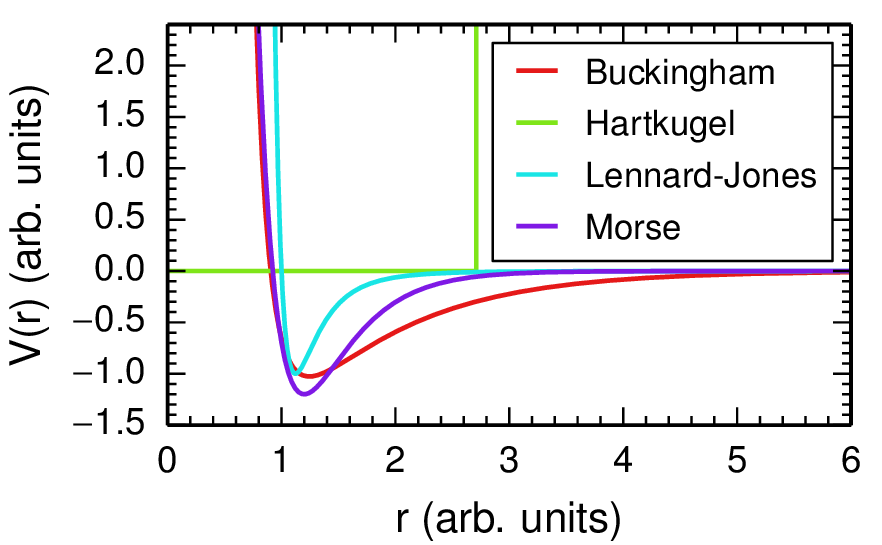
\includegraphics[width=0.5\textwidth]{mdpotplot}
  \caption{Beispiele einfacher Paarpotentiale}
  \label{fig:mdpairpotentials}
\end{figure}

Andere Potentiale enthalten weitere Parameter oder tabellierte Werte, mit denen spezielle Probleme genauer betrachtet werden können.
Das allgemeine Problem der Klasse der Paarpotentiale ist ihre Schlichtheit.
So lassen sie sich schwer an realistische Strukturen fitten und können oftmals nur ein Material in einem Szenario darstellen, wobei sie allerdings schnell sind.

\subsubsection{N-Teilchen-Potentiale}

N-Teilchen-Potentiale  erweitern Paarpotentiale um weitere Terme, die von einer festen Anzahl an Teilchen abhängen, beispielsweise Winkel- und Torsionsabhängigkeiten.

\begin{equation}
  \label{eq:nbody-energy}
  E = \sum_i\sum_{j \neq i}{V_2\left(r_{ij}\right)} + \sum_i\sum_{j \neq i}\sum_{i \neq k \neq j}{V_3\left(r_{ij}, r_{ik}, \theta_{ijk}\right)}
\end{equation}
\todo{letzte Summe: Indizes aufspalten}

Obwohl sich mit N-Teilchen-Potentialen komplexere Systeme betrachten lassen, zeigen sie die gleichen Schwachstellen wie Paarpotentiale.
Zwar gibt es erfolgreiche \todo{kommerzielle} Anpassungen für Biomoleküle (\todo{CHARMM} \todo{GROMACS} \todo{AMBER}), die allerdings nicht auf andere Stoffsysteme übertragbar sind.

\subsubsection{Embedded Atom Model}

Das Embedded Atom Model (EAM) für jedes Atom $i$ besteht aus einem Paarpotential $V_{\alpha\beta}(r_{ij})$ sowie einer Einbettungsfunktion $F_\alpha$, die die Energie jedes Atomes in Abhängigkeit der angenäherten Elektronendichte $\rho_\beta(r_{ij})$ in der Umgebung modelliert (Gleichung \ref{eq:eam-energy}).\todo{Referenz}
So lassen sich insbesondere metallische Materialien und Oberflächen simulieren.
$\alpha$ und $\beta$ stellen dabei verschiedene Atomsorten dar, allerdings lassen sich auch mit dieser umfangreicheren Formulierung hauptsächlich reine Metalle simulieren.
Für diese findet man allerdings passende Parametrisierungen\todo{Referenz auf Datenbank und passende Paper}, die im Gegensatz zu den meisten Potentialen sowohl thermodynamisches Verhalten als auch Strukturen recht gut modellieren (Abschnitt \ref{goldthermo}).

\begin{equation}
  \label{eq:eam-energy}
  E = \sum_i\left[F_\alpha\left(\sum_{j\neq i}{\rho_\beta\left(r_{ij}\right)}\right) + \frac{1}{2}\sum_{j\neq i}{V_{\alpha\beta}\left(r_{ij}\right)}\right]
\end{equation}

\subsubsection{Modified Embedded Atom Model}

Um die Einschränkung des reinen EAM-Potentials zu umgehen, wurde das Modified Embedded Atom Model (MEAM) erforscht (Gleichung \ref{eq:meam-energy}). \todo{Referenz auf Baskes}
Mit diesem lassen sich auch Metalloxide, Legierungen und andere Mischsysteme untersuchen\todo{Referenz}.

\todo{Wie funktioniert es?}

\begin{equation}
  \label{eq:meam-energy}
  E = \sum_i\left[F_\alpha\left(\bar{\rho_i}\right) + \frac{1}{2}\sum_{j\neq i}{V_{ij}\left(r_{ij}\right)}\right]
\end{equation}

Wie beim EAM-Potential sind die eigentlichen Berechnungen in den einzelnen Funktionen versteckt, die auf umfassende Weise die Elektronendichten zu modellieren versuchen.
Dafür ist vorher eine umfangreichere Parametrisierung notwendig, die an eine Vielzahl von Strukturen gefittet werden muss.

\subsubsection{Reactive Force Fields}

\todo{Referenz}
Reactive Force Fields (ReaxFF) wurden mit der Idee erdacht, bisher unmögliche Simulationen in Molekulardynamik mit größeren Systemen darstellen zu können.
Dafür fließt eine Vielzahl an Einflüssen in die Potentialparameter ein, beispielsweise Van-der-Waals-Kräfte und elektrostatische Kräfte, allerdings ist der zentrale Gedanke die Modellierung von Über- und Unterkoordination eines Atomes in seiner Nachbarschaft unter Ladungsaustausch.
Somit lassen sich Bindungen während der Simulation dynamisch formen und lösen und dadurch ganze Reaktionen zwischen verschiedenen Molekülen simulieren.

\begin{align}
  \label{eq:reax-formulation}
  E_\text{system} &= E_\text{bond} + E_\text{lp} + E_\text{over} + E_\text{under} + E_\text{val} + E_\text{pen} + E_\text{coa} + E_\text{C2} \\
  \nonumber  & + E_\text{tors} + E_\text{conj} + E_\text{H-bond} + E_\text{vdWaals} + E_\text{Coulomb}
\end{align}

Die meisten Terme der Gesamtenergie werden über die Bindungsordnung berechnet, die über Beiträge für $\sigma$-, $\pi$- und Doppel-$\pi$-Bindungen aus dem Bindungsabstand errechnet wird.
Einige werden durch Taper-Korrektur\todo{ref} in der Nähe des Cutoff-Abstandes auf 0 gesenkt, um Diskontinuitäten zu vermeiden und einen fließenden Übergang zwischen Bindungszuständen zu ermöglichen.

\todo{Referenz auf Equations\_Reax.pdf}

\begin{table}
  \begin{tabularx}{\textwidth}{|llX|}
    \hline
    \textbf{Term}      & \textbf{Beitrag}            & \textbf{Kommentar}                            \\
    \hline
    $E_\text{bond}$    & Bindungsenergien            & Berechnung über Bindungsordnung               \\
    $E_\text{lp}$      & freie Elektronenpaare       & über Bindungsordnungssumme am Atomzentrum     \\
    $E_\text{over}$    & Überkoordinationen          & unter Ausschluss freier Elektronenpaare       \\
    $E_\text{under}$   & Unterkoordinationen         & nur bei unterkoordinierten $\pi$-Bindungen    \\
    $E_\text{val}$     & Bindungswinkel              & Optimum abhängig von Elektronenkonfiguration  \\
    $E_\text{pen}$     & Strafenergien               & Fehlerkorrektur bei Winkeln mit Doppelbindung \\
    $E_\text{coa}$     & Drei-Teilchen-Konjugationen & Stabilisierung von NO$_2$-Gruppen             \\
    $E_\text{C2}$      & Dreifachbindungskorrektur   & Stabilisierung der Dreifachbindung von C$_2$  \\
    $E_\text{tors}$    & Torsionsbarrieren           &                                               \\
    $E_\text{conj}$    & Vier-Teilchen-Konjugationen & Konjugation bei Kohlenwasserstoffen           \\
    $E_\text{H-bond}$  & Wasserstoffbrücken          &                                               \\
    $E_\text{vdWaals}$ & Van-der-Waals-Kräfte        &                                               \\
    $E_\text{Coulomb}$ & Coulomb-Kräfte              &                                               \\
    \hline
  \end{tabularx}
  \caption[ReaxFF Energiebeiträge]{ReaxFF Energiebeiträge aus Gleichung \ref{eq:reax-formulation}}
  \label{tab:reax-energies}
\end{table}

Wie aus Gleichung \ref{eq:reax-formulation} und Tabelle \ref{tab:reax-energies} hervor geht, wurden das ReaxFF-Potential ursprünglich für Reaktionen von organischen Molekülen entwickelt, ist aber vielseitig genug, eine Vielzahl anderer Materialien simulieren zu können.
Die unterstützten Stoffgruppen hängen dabei stark von den Strukturen ab, an die die Parametrisierung gefittet wurde.
Auch, wenn alle notwendigen Atomsorten unterstützt werden, kommt es häufig vor, dass der zu untersuchende Stoff bei der Parametersuche nicht beachtet wurde und somit nicht darstellbar ist.

In den letzten fünf Jahren haben Reactive Force Fields jedoch langsam an Aufmerksamkeit gewonnen, so dass die Zahl spezialisierter Parametrisierungen wächst.
Es gibt auch Bestrebungen, sich ergänzende ReaxFF-Parametrisierungen zu kombinieren und somit mit einer Parametrisierung jedes gewünschte System betrachten zu können.
Besonders in kommerzieller MD-Software\todo{Referenz auf GULP} versucht man so, dem Nutzer unnötige Arbeit abzunehmen.
Es muss sich jedoch noch zeigen, ob dieser Ansatz zufrieden stellende Ergebnisse liefern kann.

\subsubsection{Allgemeine Probleme}

\textbf{Parametrisierung}:
Da Molekulardynamik keine ab-initio-Methode ist, sondern jedes Potential erst an experimentelle oder numerische Daten angepasst (gefittet)\todo{was nun?} werden muss, sollte die Herkunft jeder Parametrisierung bei seiner Nutzung bedacht werden.
\todo{kulkarni: Kritische Betrachtung seiner Trainingsstrukturen}
\\\\
\textbf{Übertragbarkeit}:
Je nach Potentialart lassen sich viele Parametrisierungen nicht vermischen oder auf andere Probleme übertragen.
\\\\
\textbf{Analysemethoden}:
Im Normalfall sind Potentiale entweder für strukturelle oder thermodynamische Größen optimiert.
Mit einem rein strukturellen Potential lassen sich also keine thermodynamischen Größen und Phasenübergänge verlässlich ermitteln.
\\\\
\textbf{Reaktionen}:
Mit der Ausnahme des ReaxFF-Potentiales lassen sich per Molekulardynamik keine Reaktionen betrachten.
\\\\
\textbf{Annäherungen}:
\todo{Was hast du hier gedacht, Erik?}

\subsection{Auswertung}

\subsubsection{Relaxierungen}

\subsubsection{Struktur}

Zur Auswertung einer Struktur bietet sich zuerst eine visuelle Beurteilung an, die mit entsprechenden Programmen vorgenommen werden kann.
Damit können grobe Defekte ausgeschlossen werden.

\subsubsection{Dichte}

Die Dichte lässt sich bei periodischen Strukturen nach über Volumen und

\subsubsection{Radiale Verteilungsfunktionen}

\subsubsection{Oberfläche}

Die Oberfläche einer Struktur gibt Hinweise auf angelagerte Moleküle, Rauheit, Porösität und Bildung von Cluster und Nanopartikeln.
Bei großen, glatten Strukturen reicht oft ein Schnitt entlang einer Hauptachse, um Bulk und Oberfläche zu trennen.
In den verbliebenen Fällen lässt sich zu diesem Zweck eine Alpha-Form per Delaunay-Triangulation bestimmen (Abschnitt \ref{datadelaunay}.
Die eigentlichen Untersuchungen beschränken sich dann auf eine Zählung der Bindungen und Atomsorten, Radiale Verteilungsfunktionen, Messungen der Oberfläche oder Abweichungen der Schichtdicke vom Mittelwert.

\subsubsection{Reaktionen}



\subsection{Software}

Für molekulardynamische Simulationen gibt es sowohl kommerzielle als auch freie Softwarepakete, die einige Parametersätze mitbringen.
Tabelle \ref{tab:mdsoftware} stellt eine Auswahl daraus dar.

\begin{table}
  \oddrowcolors
  \caption[MD-Software]{MD-Software}
  \label{tab:mdsoftware}
  \begin{tabularx}{\textwidth}{|llX|}
    \hline
    \textbf{Paket} & \textbf{Rechteinhaber} & \textbf{Kommentare} \\
    \hline
    LAMMPS & SANDIA & quelloffen, CLI-bedienbar, Bibliothek, eigene Potentiale möglich \\
    Materials Studio GULP & Accelrys & Tief in graphischer Oberfläche verankert \\
    AMBER & University of California & verschiedene Biomoleküle \\
    CHARMM & Accelrys & Proteine \\
    GROMACS & Uppsala University & Biomoleküle, quelloffen \\
    \hline
  \end{tabularx}
  \todo[inline]{References!}
  \todo[inline]{bessere Beschreibung!}
\end{table}

